\documentclass[10pt]{article}
\usepackage[utf8]{inputenc}
\usepackage[landscape,paper=ansibpaper]{geometry}
\usepackage{tikz}
\usetikzlibrary{trees}
\usetikzlibrary{shadings}
\tikzstyle{every node}=[draw=black,thin,anchor=west, minimum height=3em]

\begin{document}

\begin{figure}[!htb]
\resizebox{\linewidth}{!}{

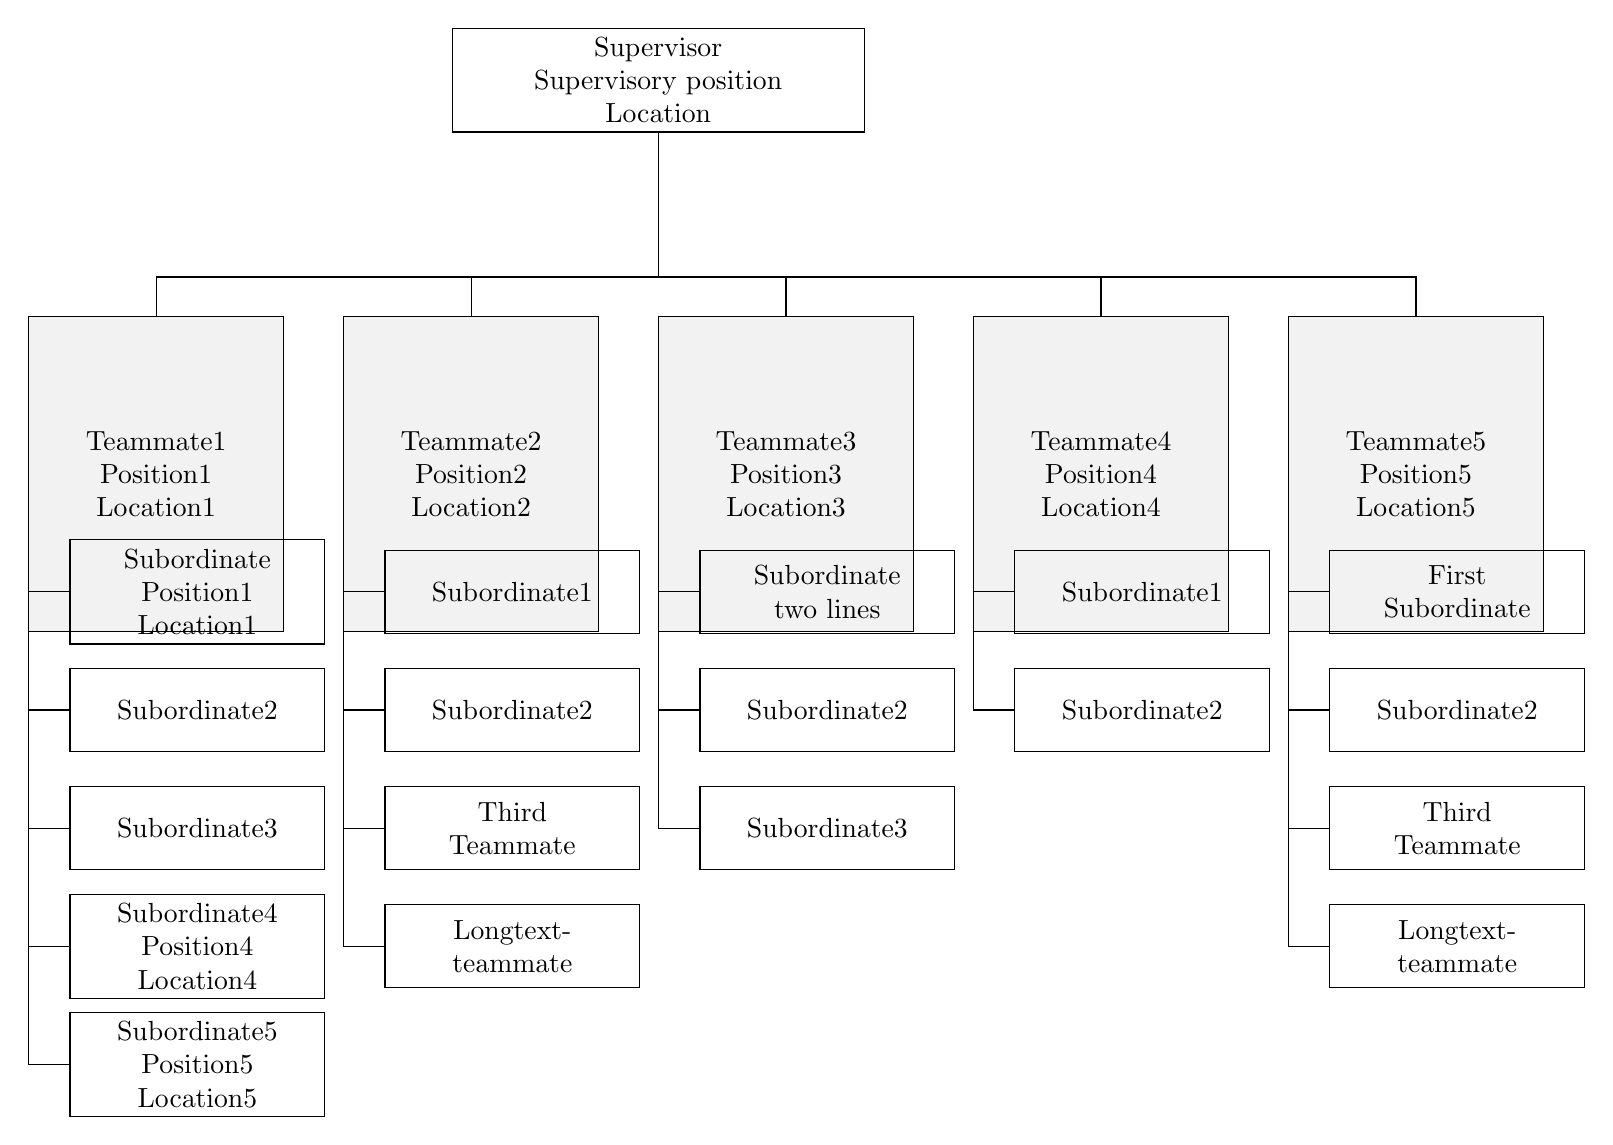
\begin{tikzpicture}[
    supervisor/.style={%
        edge from parent fork down,
        level distance=2.5cm,
        text centered, text width=5cm},
    teammate/.style={%
        text centered, text width=3cm,
        level distance=2.5cm,
        minimum height=4cm,
        fill=gray!10},
    subordinate/.style={%
        grow=down, xshift=-1.1cm, % Horizontal position of the child node
        text centered, text width=3cm,
        edge from parent path={(\tikzparentnode.205) |- (\tikzchildnode.west)}},
    level1/.style ={level distance=1.5cm},
    level2/.style ={level distance=3cm},
    level3/.style ={level distance=4.5cm},
    level4/.style ={level distance=6cm},
    level5/.style ={level distance=7.5cm},
    level 1/.style={sibling distance=4cm},
    level 1/.append style={level distance=5cm},
]
%   \draw[help lines] (0,0) grid (4,3);

    % Supervisor
    \node[anchor=south,supervisor]{Supervisor\\Supervisory position\\Location}
    [edge from parent fork down]

    % Teammate and Subordinates
    child{node [teammate] {Teammate1\\Position1\\Location1}
        child[subordinate,level1] {node {Subordinate\\Position1\\Location1}}
        child[subordinate,level2] {node {Subordinate2}}
        child[subordinate,level3] {node {Subordinate3}}
        child[subordinate,level4] {node {Subordinate4\\Position4\\Location4}}
        child[subordinate,level5] {node {Subordinate5\\Position5\\Location5}}}
    %
    child{node [teammate] {Teammate2\\Position2\\Location2}
        child[subordinate,level1] {node {Subordinate1}}
        child[subordinate,level2] {node {Subordinate2}}
        child[subordinate,level3] {node {Third\\Teammate}}
        child[subordinate,level4] {node {Longtext-\\teammate}}}
    %
    child{node [teammate] {Teammate3\\Position3\\Location3}
        child[subordinate,level1] {node {Subordinate\\two lines}}
        child[subordinate,level2] {node {Subordinate2}}
        child[subordinate,level3] {node {Subordinate3}}}
    %
    child{node [teammate] {Teammate4\\Position4\\Location4}
        child[subordinate,level1] {node {Subordinate1}}
        child[subordinate,level2] {node {Subordinate2}}}
    %
    child{node [teammate] {Teammate5\\Position5\\Location5}
        child[subordinate,level1] {node {First\\Subordinate}}
        child[subordinate,level2] {node {Subordinate2}}
        child[subordinate,level3] {node {Third\\Teammate}}
        child[subordinate,level4] {node {Longtext-\\teammate}}};

%\shade[shading=Mandelbrot set] (0,0) rectangle (5,5);
\end{tikzpicture}}
\caption{This is an org chart}
\end{figure}

\end{document}